\documentclass[12pt]{scrartcl}

\usepackage[utf8]{inputenc} % utf8 encoding
\usepackage[T2A]{fontenc}
\usepackage[english,russian]{babel}
\usepackage{cmap}

%\usepackage{fontspec}
%\usepackage{polyglossia}
%\setdefaultlanguage{russian}
%\newcommand{\docfont}{Times New Roman}
%\setmainfont[Ligatures=TeX]{\docfont}
%\newfontfamily\cyrillicfont[Ligatures=TeX]{\docfont}
%\newfontfamily\cyrillicfontsf[Ligatures=TeX]{\docfont}
%\newfontfamily\cyrillicfonttt[Ligatures=TeX]{\docfont}

\usepackage{amsmath,amsfonts,amsthm,amssymb} % nice math symbols
\newtheorem{definition}{Определение}
\usepackage{hyperref}

\hypersetup{%
	pdfencoding=auto,
	pdfauthor={Александр Панов},
	pdftitle={Отношения и операции в знаковой картине мира субъекта поведения}
}
\usepackage{csquotes}
\usepackage{graphicx}
\graphicspath{{../../images/}}

\usepackage[plain]{algorithm}
\usepackage[noend]{algpseudocode}
\renewcommand{\algorithmiccomment}[1]{{\quad\footnotesize // #1}}
\renewcommand{\algorithmicrequire}{\textbf{Input:}}
\renewcommand{\algorithmicensure}{\textbf{Output:}}

\usepackage[
	autolang=hyphen,
	language=auto,
	autolang=other,
	backend=biber,
	style=gost-numeric
]{biblatex}
\addbibresource{operations.bib}
\DeclareSourcemap{
	\maps[datatype=bibtex, overwrite]{
		\map{
			\step[fieldset=langid, fieldvalue=english]
			\step[fieldset=doi, null]
			\step[fieldset=issn, null]
			\step[fieldset=isbn, null]
			\step[fieldset=url, null]
			\step[fieldsource=language, fieldset=langid, origfieldval]
		}
	}
}

\newcommand{\linesprval}{1}
\linespread{\linesprval}
%\renewcommand\arraystretch{0.5}
\floatplacement{figure}{H}

\title{Отношения и операции в знаковой картине мира субъекта поведения}
\author{Г.\,С.~Осипов, А.\,И.~Панов\\
	{\large\slshape ФИЦ ИУ РАН, пр. 60-летия Октября, 9, gos@isa.ru}}

\begin{document}
%	\affil{ФИЦ ИУ РАН}
	
	\maketitle{}
	\begin{abstract}
		В соответствии с современными взглядами на возникновение психических функций и на роль в этом  нейрофизиологических процессов, формирование психических функций связывается с существованием или синтезом в процессе коммуникации специальных информационных структур, содержащих три различных по происхождению вида информации: информации, поступающей из внешней среды, информации, извлекаемой из памяти, и информации, приходящей из центров мотивации. Связывание таких компонент в единое целое обеспечивается их именованием; оно же обеспечивает устойчивость возникающих структур. Такие информационные структуры были названы нами знаками ввиду их сходства с аналогичными структурами, изучаемыми в семиотике. Множество знаков, формируемых субъектом в процессе деятельности и коммуникации, образует его знаковую картину мира, отражающую его представления о внешней среде, о себе и о других субъектах.
		
		Знаковая картина мира позволяет поставить и решить ряд задач, возникающих при моделировании поведения интеллектуальных агентов и их коалиций, таких как задачи целеполагания, синтеза целенаправленного поведения, распределения ролей и взаимодействия агентов в коалиции. В работе рассматривается специальный объект - каузальная матрица, с помощью которой описывается строение компонент знака. На этой основе определяются операции и отношения в знаковой картине мира, моделирующие психологические особенности поведения человека. 
		
		\par\bigskip
		\textit{Ключевые слова}: знаковая картина мира, образ, значение, личностный смысл, каузальная матрица, семиотическая сеть, обобщение.
	\end{abstract}
	
	
	\section*{Введение}
	Проблема возникновения ощущений является, видимо, одной из центральных проблем когнитивной психологии. Нет ясности и в связи этого феномена с формированием картины мира субъекта. В работах таких психологов как А.Н. Леонтьев \cite{Leontiev1977}, представление каждого объекта или явления действительности в сознании включает три компонента: образ объекта, культурно-историческое значение и его личностный смысл. В соответствии с понятием образа, развиваемым в когнитивной психологии, восприятие рассматривается как процесс категоризации, значение соответствует предназначению объекта, семантической компоненте знака, и личностный смысл интерпретируется как множество действий с объектом, предпочитаемых субъектом. Такая структура, как легко видеть, близка к структуре, именуемой в семиотике знаком \cite{Pierce2000b,Frege2000}, поэтому подход, культивируемый в настоящей работе уместно назвать знаковым или семиотическим. В пользу описанной выше структуры картины мира свидетельствует не только культурно-исторический подход, но и другие психологические теории, в частности трехпроцессная модель Станович \cite{Stanovich2009}. В ней, в отличие от известной двухпроцессной модели Канемана \cite{Kahneman2011} психические процессы реализуются тремя подсистемами: рефлексивной, алгоритмической и автономной.
	
	Эти соображения подтверждаются результатами многих исследований и в области нейрофизиологии, прежде всего \cite{Ivanitsky1996}, в соответствии с которыми возникновение ощущения, т.е. переход с нейрофизиологического уровня на психологический, связывается с кольцевым движением возбуждения отделов коры мозга, которое после дополнительной обработки в других структурах мозга возвращается к местам первоначальных проекций сигнала (<<круг ощущений>>). Психическая функция \cite{Ivanitsky2010} возникает на основе синтеза трёх видов информации (т.е., по существу, с формированием трёхкомпонентных структур): информации, исходящей из внешней среды (сенсорной), извлекаемой из памяти и приходящей из центров мотивации. Следует заметить, что работы \cite{Edelmen1981,Edelman1987} также свидетельствуют о возможности существования знаковых структур в картинах мира субъектов деятельности. В \cite{Friederici2015} рассмотрен механизм формирования некоторых когнитивных функций и его связь с формированием языковой модели мира. Работа \cite{Loula2012} посвящена возникновению механизмов коммуникации на основе семиотического подхода. В \cite{Roy2005} Рой предложил знаковую модель мира как основу операционной компоненты робота. 
	
	В последующие годы использование идеи возврата возбуждения для объяснения механизмов сознания и <<знаковую>> гипотезу подтвердили результаты многих исследований, в том числе данные о строении отделов мозга, входящих в <<круг ощущений>>. Компоненты знака находят свою нейронную реализацию в различных подсистемах мозга. Образная компонент знака реализуется процессами распространения нейронной активации от первичных сенсорных отделов кортико-таламической системы к ассоциативным.  При этом исследователи разделяют два пути  активации: нижний (вентральный), определяющий пространственно независимые объектные характеристики поступающей сенсорной информации, и задний (дорзальный), распознающий пространственную конфигурацию и действия \cite{Grossberg2014}. Существование этих двух активационных потоков оправдывает существование объектных и процедурных признаков в образной компоненте знака (раздел \ref{sec:structure}).
	
	Наличие обратной связи в процессе распознавании образов, играющей роль предсказывающей предактивации нейронов (подробнее в разд. \ref{subsec:actual}), создает эффект повторного входа в первичные отделы коры \cite{Edelmen1981,Ivanitsky1996}. Компонента личностного смысла является продуктом взаимодействия моторных отделов коры и таких подкорковых структур как таламус, базальные ядра, миндалевидное тело и гипоталамус. Именно этими подсистемами мозга реализуется интеграция предыдущего опыта действования и выбор действия в текущей ситуации с учетом текущего мотива и цели \cite{Gurney2001}. Тесно связан с компонентой личностного смысла и гиппокамп, который играет важную роль в формировании эпизодической памяти, т.е. описании текущей и недавних ситуаций деятельности \cite{Rolls2010}. Наконец, компонента значения является результатом обобщающей и абстрагирующей функции мозга и реализуется лобными и верхними височными отделами коры мозга. В этих же отделах происходит и связывание всех компонент знака с их последующим именованием \cite{Friederici2015,Pulvermuller2013}.

	В разд. \ref{sec:sintaxis} будет описана высокоуровневая, концептуальная часть модели, в которой мы не углубляемся в детали строения знака и описываем общую схему его формирования и его синтаксическое определение. В разд. \ref{sec:semantic} приводится интерпретация компонент знака с использованием логики предикатов и системы правил (операциональная семантика). Далее основное внимание будет уделено нейрофизиологически и психологически правдоподобной модели знака, его структуре (разд. \ref{sec:structure}). На этом структурном уровне будут предложены основные математические объекты и даны определения компонент знака, описан алгоритм работы образной компоненты. Далее дается структурное определение семействам базовых отношений на компонентах знака и вводится понятие семиотической сети как модели картины мира (разд. \ref{sec:semnetwork}). В качестве демонстрации применимости построенной модели в разд. \ref{sec:operations} описываются основные операции в картине мира, которые моделируют известные когнитивные функции: обобщение, образование сценария и агглютинация смыслов.
	
	\section{Синтаксический уровень}\label{sec:sintaxis}

	Определим синтаксический уровень модели картины мира, следуя работам \cite{Osipov2014c,Osipov2016c}.Пусть задано множество $S$, которое будем называть множеством знаков. Каждый элемент $s\in S$ имеет вид $s=\langle n,p,m,a\rangle$, где $n\in N$, $p\subseteq P$, $a\subseteq A$, $m\subseteq M$. Здесь $N$ --- множество слов конечной длины в некотором алфавите, которое будем называть множеством имен; $P$ --- множество замкнутых атомарных формул языка исчисления предикатов первого порядка, которое будем называть множеством свойств; $M$ будем называть множеством значений; $A$ — множеством смыслов. Как множество значений $M$, так и множество смыслов $A$, поскольку это следует из психологических соображений, интерпретируется множеством действий. Каждое действие, как это принято в искусственном интеллекте, представим с помощью правила \cite{Osipov2008b}. Правилом называется упорядоченная тройка множеств:	$r=\langle Con,Add,Del\rangle$, где $Con$ --- условие правила; $Add$ --- множество фактов, добавляемых правилом $r$; $Del$ --- множество фактов, удаляемых правилом $r$. Каждое из этих множеств, в общем случае, есть множество атомарных формул исчисления предикатов первого порядка. Более детально указанные роль правил в знаковой модели будет описана в следующем разделе.
	
	Введем далее операторы связывания. $\Psi_p^m:2^P\rightarrow 2^M$ --- оператор связывания образов $p$ со значениями $m$. Второй оператор $\Psi_m^a:2^M\rightarrow 2^A$ связывает значения со	смыслами. Третий оператор $\Psi_a^p: 2^A\rightarrow 2^P$ связывает смыслы с образами. Введенные операторы связывают компоненты знак друг с другом, а их семантика определятся в следующем разделе. На синтаксическом уровне модели определяются основные алгоритмы: формирование знака и процедуры самоорганизации \cite{Osipov2014c}.
		

	\section{Семантический уровень модели}\label{sec:semantic}
	
	На семантическом уровне модели картины мира уточняется операционная семантика введенных на синтаксическом уровне операторов связывания, а компоненты знака интерпретируются символами исчисления предикатов и правилами, как они определяются в искусственном интеллекте \cite{Osipov2015c,Osipov2016a}.
	
	Определим оператор связывания (рис. \ref{fig:linkers}) $\Psi_p^m(p^{(i)})=m^{(i)}$, так что $m^{(i)}=\{r|\mathcal{P}_c(r)\subseteq \mathcal{P}(p^{(i)})\}$, где $\mathcal{P}_c(r)$ --- множество различных предикатных символов условия $Con$ правила $r$, интерпретирующего значение $m$ (здесь и далее для простоты мы будем с каждым значением связывать ровно одно действие, т.е. одно правило); $\mathcal{P}(p^{(i)})$ --- множество предикатных символов образа $p^{(i)}$; $p^{(i)}\in 2^P$ , $m^{(i)}\in 2^M$ , $2^P$ и $2^M$ --- булеаны $P$ и $M$ соответственно. 
	
	\begin{figure}
		\label{fig:linkers}
		\centering
		\includegraphics[width=0.32\textwidth,page=1]{sign-schemas/oper_relat}
		\includegraphics[width=0.32\textwidth,page=2]{sign-schemas/oper_relat}
		\includegraphics[width=0.32\textwidth,page=3]{sign-schemas/oper_relat}
		\caption{Операторы связывания компонент знака.}		
	\end{figure}
	
	Второй оператор	$\Psi_m^a(m^{(i)})=a^{(i)}$, где $a^{(i)}=\{r^*|\mathcal{P}_c(r)\cap \mathcal{P}_c(r^*)\not=\varnothing\}$, где $\mathcal{P}_c(r)$ --- множество предикатных символов условия $Con$ правила $r^*$, интерпретирующего личностный смысл $a^{(i)}$ (здесь, как и в случае со значением, для простоты, с каждым личностным смыслом связывается ровно одно действие, т.е. одно правило); $m^{(i)}\in 2^M, a^{(i)}\in 2^A$, $2^A$ --- булеан $A$. Третий оператор $\Psi_a^p(a^{(i)})=p^{(i+1)}$, где $p^{(i+1)}\subseteq \mathcal{P}_a(r_j^*)$, $a^{(i)}\in 2^A$, $p^{(i+1)}\in 2^P$, где $\mathcal{P}_a(r_j^*)$ --- множество предикатных символов из множества добавлений правила $r_j^*$.
	
	Разумеется, $p^{(i)}\not = p^{(i+1)}$. Можно показать, что при определенном начальном приближении этот итеративный процесс сходится к некоторому $p$. При этом $\|\mathcal P_c(r)\cap\mathcal P_c(r^*)\|\geq 2$. Легко видеть, что достаточным условием сходимости является $\mathcal P_c(r)\subseteq\mathcal P_c(r^*)$. Если ввести оператор $\Psi_m^p=\Psi_a^p\Psi_m^a$, то легко видеть, что пара операторов $\Psi_p^m$ и $\Psi_m^p$ образуют соответствие Галуа, а знак есть неподвижная точка замыкания Галуа операторов $\Psi_p^m$ и $\Psi_m^p$.
	
	На семантическом уровне модели картины мира становится возможным описать отношения на множестве компонент знаков: отношения на множестве образов, значений и личностных смыслов. Каждое отношение из этих семейств может быть транслировано на множество имен, что позволяет уже определить отношения на множестве знаков. Далее приведем семантические определения ряда этих отношений, а также операций на множестве знаков. Далее на структурном уровне все отношения и операции будут уточнены при рассмотрении структуры компонент знака.
		
	\subsection{Операции и отношения на множестве знаков}
	Пусть $S=\{s_1,s_2,\dots,s_k\}$ "--- множество знаков, $p_1=(x_1,x_2,\dots,x_g)$ и $p_2=(y_1,y_2,\dots,y_h)$ "--- образы знаков $s_1$ и $s_2$, $x_i$ - значение $i$-го признака. Упорядоченные множества $\tau_1=\langle i_1,i_2,\dots,i_g\rangle$ и $\tau_2=\langle j_1,j_2,\dots,j_h\rangle$, где $i_1,i_2,\dots,i_p\in\{1,\dots,g\}$, $j_1,j_2,\dots,j_q\in\{1\dots,h\}$, будем называть типами образов знаков $s_1$ и $s_2$ соответственно.
		
	\begin{definition}
		Если для знаков $s_1$ и $s_2$ $\tau_1=\tau_2$ и $x_i=y_i$, то $R^p_{eq}:=R^p_{eq}\cup\{(s_1,s_2)\}$, $R^p_{eq}\subseteq S\times S$.
	\end{definition}

	Легко видеть, что отношение $R^p_{eq}$ - это отношение эквивалентности на множестве образов знаков из $S$. Определенные ниже отношения $R^p_{in}$, $R^p_{sim}$, $R^p_{con}$ - отношения включения, сходства и противопоставления соответственно.

	\begin{definition}
		 Если для знаков $s_1$ и $s_2$ $\tau_1\subset\tau_2$ и $\forall i\in\tau_1$ имеет место $x_i=y_i$, то $R^p_{in}:=R^p_{in}\cup\{(s_1,s_2)\}$, $R^p_{in}\subseteq S\times S$.
	\end{definition}
	
	\begin{definition}
		Если для знаков $s_1$ и $s_2$ $\tau_1\cap\tau_2\not =\varnothing$ и $\forall i\in(\tau_1\cap\tau_2)$ имеет место $x_i=y_i$, то $R^p_{sim}:=R^p_{sim}\cup\{(s_1,s_2)\}$, $R_3\subseteq S\times S$.
	\end{definition}
	
	\begin{definition}
		Если для знаков $s_1$ и $s_2$ $\tau_1\cap\tau_2\not =\varnothing$ и $\forall i\in(\tau_1\cap\tau_2)$ имеет место $x_i\not =y_i$, то $R^p_{con}:=R^p_{con}\cup\{(s_1,s_2)\}$, $R^p_{con}\subseteq S\times S$.
	\end{definition}

	Приведённые определения являются процедурами порождения новых элементов отношений на множестве знаков. Запускаясь всякий раз, когда множество знаков пополняется новым знаком (или когда множество знаков начинает использоваться), описанные процедуры либо формируют новое отношение, либо пополняют какое-либо из отношений на знаках новым элементом.
	
	Операция обобщения $\Theta^p$ определена на множестве пар знаков, принадлежащих отношению $R^p_{sim}$; результат работ $\Theta^p$ - новый образ, включающий все общие признаки исходных образов. А именно, если $P$ - множество образов, $p_1\subset P,p_2\subset P$, $p_1=(x_1,x_2,\dots,x_g), p_2=(y_1,y_2,\dots,y_h)$, тогда $\Theta:P\times P\rightarrow P$ так, что для всяких $p_1,p_2$ таких, что $(s_1,s_2)\in R^p_{sim}, \Theta^p(p_1,p_2)=p_3$, где $p_3=(z_1,z_2,\dots, z_l)$, так, что для $\forall i\exists j,k$ такие, что $z_i=x_j=y_k$. Сформированный в результате обобщения образ может служить основой для формирования нового знака.
	
	Переходя к значениям знаков, необходимо напомнить, что значение есть множество обобщенных действий, которые субъект может выполнять с предметом, представляемым некоторым знаком. Однако всякому действию соответствует набор некоторых ролей, которые замещаются участниками рассматриваемого действия, примерно так, как это описано у Филмора \cite{Fillmore1988}. Таким образом, со значением каждого знака будет связано некоторое упорядоченное множество, которое называется набором его ролей. Понятно, что каждая роль также может замещаться некоторым знаком. Эти соображения лежат в основе формирования отношения на множестве знаков, порождаемого значениями последних, которое уместно назвать сценарным. 
	
	Итак, если $I=\{i_1,i_2,\dots,i_q\}$ - множество всех возможных	ролей, то значение каждого знака есть некоторое подмножество этого множества. Для простоты будем здесь полагать, что каждое значение содержит одно действие. Пусть теперь $s_1, s_2$ - знаки, $m(s_1)=\langle i_1,i_2,\dots,i_k \rangle$ - значение знака $s_1$, где $i_1,i_2,\dots,i_k\in I$.
	
	\begin{definition}
		Если для знаков $s_1$ $s_2$ имеет место $s_2 / i_j$	(знак $s_2$ замещает роль $i_j$), $i_j\in m(s_1)$, то $R^m_{sc}:=R^m_{sc}\cup\{(s_1,s_2)\}$.
	\end{definition}
	
	Это отношение уместно назвать сценарным, так как оно позволяет порождать сложные конструкции -  сценарии, которые суть сети знаков, связанных посредством значений и имен последних. На семантическом уровне возможно ввести еще ряд отношений, порождаемых значениями и личностными смыслами \cite{Osipov2014c}.
	
	Дадим определение операция замыкания по значениям $\Theta^m(s_1,i_j,s_2)$. Если $s_1$ - знак со значением $m(s_1)$ и $i_j\in m(s_1)$ - одна из ролей этого значения, то операция строит новый знак $s^*$, в котором роль $i_j$ замещена знаком $s_2$ ($s_2/i_j$). При этом образы, смыслы и значения исходных знаков объединяются.
	
	На основе личностных смыслов на множествах знаков естественным образом порождаются отношения поглощения и противопоставления \cite{Osipov2014c}. Напомним, что всякому смыслу соответствует некоторое множество специфицированных (конкретизированных) действий. 

	Введем операцию агглютинации $\Theta^a(s_1,s_2)=s_3$. Здесь для простоты, как и выше, положим, что каждому смыслу соответствует одно действие, которое описывается правилом $\langle Con, Add, Del \rangle$. Если $s_1,s_2$ - знаки, a $a_1,a_2$ - их смыслы, то операция агглютинации формирует	новый знак $s_3$ со смыслом $a_3$, где $Add(r_3)=Add(r_1)\cup Add(r_2)$ либо $Del(r_3)=Del(r_1)\cup Del(r_2)$. Понятно, что в обоих случаях $Con(r_3)=Con(r_1)\cap Con(r_2)$, где $Con$ - множества условий правил $r_1,r_2,r_3$, $Add$ и $Del$ - множества фактов, добавляемых и удаляемых соответствующими правилами.
		
	
	\section{Структурный уровень модели}\label{sec:structure}
	
	Далее мы остановимся на структурной модели компонент знака, которая учитывает современные нейрофизиологические данные о строении кортико-таламической подсистемы мозга и механизмах передачи активации между отделами коры. Множество предикатных символов $\mathcal P(\cdot)$ будет заменено множеством признаков, организованных в специальные структуры (каузальные матрицы), которые в свою очередь составляют каузальную сеть. Объединение признаков (предикатных символов) в такие структуры позволяет с помощью единого формализма описывать как образную компоненту знака (множество предикатных символов), так и значение и личностные смыслы (правила с эффектами и условиями).
	
	Рассмотрим структуру компонент знака на примере образной компоненты, которая участвует в распознавании представляемого объекта или процесса на основе поступающей из внешней среды сенсорной информации и регистрируемой внутренними сенсорами моторной информации (в результате распознавания образа знака происходит актуализация знака). До именования знак будем называть протознаком или признаком.
	
	Предположим, что во входном потоке данных выделена последовательность $(x_1,x_2,\dots,x_h)$ длины $h$ векторов $x_i$ действительных чисел от 0 до 1, которые будем называться \textit{событиями}. Каждое событие $x_t$ длины $q$ представляет собой запись выходов от $q$ сенсоров, а каждый элемент события означает степень уверенности (субъективную вероятность в байесовском смысле) в срабатывании соответствующего сенсора. Например, событие $(0.1, 0.9, 0.9)$ поступает с трех сенсоров - датчиков красного, синего и зеленого света - и означает, что степень уверенности в срабатывании датчика красного света составляет $0.1$, а синего и зеленого --- по $0.9$.
	
	Образная компонента знака отвечает в первую очередь за распознавание представляемого объекта на основе входной информации. В процессе функционирования образа знака используется или строится специальная распознающая функция, принимающая на вход последовательность векторов, содержащих информацию о признаках объекта в отдельные моменты времени. Распознающая функция определяет, присутствует ли (закодирован ли) представляемый знаком объект в этой последовательности. Далее будем считать, что данная функция уже построена в результате специального процесса обучения (подробнее \cite{Panov2014d,Skrynnik2016}).
	
	Будем представлять распознающую функцию (т.е. кодировать характерные признаки объекта или процесса) специальной структурой - каузальной матрицей $z=(e_1,e_2,\dots,e_h)$ размерности $q$ на $h$, где $q$ - размерность событий (количество сенсоров), а $h$ - длина последовательности событий. При этом каждый столбец $e_t$ каузальной матрицы является бинарным вектором длины $q$ и кодирует те признаки (которым соответствуют 1), которые необходимо должны присутствовать во входном событии в момент времени $t$, чтобы представляемый объект или процесс мог быть распознан во входном потоке данных, т.е. задают множество одновременных характерных признаков. Например, образу знака $s$, представляющему объект <<лицо>>, может соответствовать каузальная матрица 	
	\[
		z=\begin{bmatrix}
			1 & 0 & 0 & 0\\
			0 & 1 & 0 & 0\\
			0 & 0 & 1 & 0\\
			0 & 0 & 0 & 1\\
		\end{bmatrix},
	\]
	где первая строка является характеристическим вектором информации с датчика левого глаза на изображении, вторая - с датчика правого глаза, третья - носа, четвертая - рта (рис.\ref{fig:face}).

	\begin{figure}
		\label{fig:face}
		\centering
		\includegraphics[width=0.5\textwidth]{misc/photos/face}
		\caption{Визуальная интерпретация каузальной матрицы. 1 обозначена область детектирования сенсора, отвечающего за левый глаз, 2 - за правый глаз, 3 - за нос и 4 - за рот. Стрелками обозначены временные переходы (саккады) от срабатывания одного сенсора к срабатыванию следующего.}		
	\end{figure}

	В вышеприведенном примере, каждый признак, составляющий образ знака <<лицо>>, также может представляться некоторым знаком в картине мира субъекта. Таким образом, случай, когда характерными признаками образа знака выступают данные с сенсоров, является частным. В более общей постановке, признаками, образующими образ знака, являются другие знаки, которые соответствуют этим характерным признакам. Следовательно, мы можем сопоставить образу $p$ знака $s$ множество $S_p(s)$ мощности $q$, каждому элементу которого соответствует номер строки каузальной матрицы $z$ размера $q$ на $h$, т.е. каждому признаку $s_i\in S_p(s)$ соответствует характеристический бинарный вектор, задающий на местах единиц те дискретные моменты времени, в которые данный признак должен присутствовать во входных данных, чтобы успешно распознать образ знака (актуализировать знак) $s$. 
	
	Образу каждого знака может соответствовать несколько каузальных матриц, которые задают различные прецеденты наблюдения во внешней среде представляемого объекта или процесса. Весь кортеж каузальных матриц образа знака $s$ будем обозначать как $Z^p(s)$. 
		
	Для уточнения определения множества $S_p(s)$ введем семейство вложенных бинарных отношений $\{\sqsubset_p,\sqsubset_p^1,\sqsubset_p^2,\dots\}$, определённых на множестве знаков $S$. Будем считать, что знак $s_i$ \textit{является элементом образа} знака $s$, $(s_i,s)\in\sqsubset_p$ или $s_i\sqsubset_p s$, в том случае, если $s_i\in S_p(s)$. Если известно, что знаку $s_i$ соответствует единица в $t$-м столбце некоторой каузальной матрицы $z\in Z^p(s)$ знака $s$, то будем использовать отношение $\sqsubset_p^t$ такое, что  $\sqsubset_p^t\subset \sqsubset_p$.
	
	\subsection{Функция распознавания образа знака}\label{subsec:actual}
	
	Кратко опишем работу алгоритма распознавания образа знака (актуализации знака) по рис.~\ref{fig:percept}. Будем считать, что образы знаков сгруппированы по сходству множеств $S_p(s)$ в узлы, которые организованы в иерархические структуры (подробнее \cite{Panov2014d}). В узлы нижнего уровня входят каузальные матрицы знаков, которые являются признаками для знаков, чьи каузальные матрицы входят в узлы более высокого уровня. Такие узлы и каузальные матрицы образов знаков формируются в результате обучения \cite{Panov2014d,Skrynnik2016}, в данной версии алгоритма мы считаем, что все матрицы и узлы уже сформированы и не обновляются. Далее ограничимся тем случаем, когда все матрицы в рамках одного узла обладают одним и тем же количеством столбцов, что в ввиду схожести матриц в одном узле является естественным условием. Промежуток времени, в течение которого обрабатываются все колонки каузальных матриц узла называется вычислительным циклом данного узла.
	
	\begin{figure}
		\centering
		\includegraphics[width=0.8\textwidth]{algo/perception}
		\caption{Схема алгоритма распознавания образа знака}
		\label{fig:percept}		
	\end{figure}

	Входными данными для алгоритма является некоторое начальное время $\tau_s$, вектор предсказаний распознаваемых признаков на данном уровне иерархии $\hat x^{j+1}(\tau_s)$ и функция входов $\omega^j$, задающая последовательность входных векторов событий $\bar x(t)$. В результате работы алгоритма формируется функция выходов $\vec \eta^j$ - последовательность векторов распознаваемых признаков и функция ожиданий - последовательность векторов событий - предсказаний распознаваемых признаков для нижнего уровня иерархии.

	\linespread{1}
	\begin{algorithm}[H]
		\label{alg:automato}
		\begin{algorithmic}[1]
			\input{../../algorithms/alg_perc_init}
			\algstore{algst:store1}
		\end{algorithmic}
	\end{algorithm}
	\linespread{\linesprval}
	
	Вычислительный цикл распознавания в узле уровня $j$ начинается с определения начального состояния узла при помощи действительного вектора с верхнего уровня иерархии - вектора ожиданий $\hat x^{j+1}(\tau_s)$, формируемого на основе состояния узла верхнего уровня (шаги \ref{alst:init_start}--\ref{alst:init_end}) в момент времени $\tau_s$. Начальное состояние определяется как подмножество таких знаков, образы которых предсказываются на основе вектора ожиданий. Введем некоторую константу $c_1$, которая определяет порог предсказываемого веса распознаваемых образов, выше которого соответствующие каузальные матрицы попадают во множество активных матриц $Z^*$ (шаг \ref{alst:select_f}). Далее производится отбор тех каузальных матриц из множества активных, для которых обычное расстояние по норме $\|x\|=\sum_i |x_i|$ первого столбца $e_1$ от события $\bar x^j(0)$ в начальный момент времени не превышает некоторой константы $c_2$ (шаг \ref{alst:select_z}). Обновленное множество полученных таким образом активных каузальных матриц является текущим состоянием узла (шаг \ref{alst:init_state}). На основе активных каузальных матриц методом голосования вычисляется выходной вектор узла  в начальный момент времени $\tilde x^j(0)$ (шаги \ref{alst:init_calc_out2} -- \ref{alst:init_calc_out3}).

	Вектор ожиданий $\hat x^j(0)$ определяется как нормированный вектор, $s$-ый компонент которого равен сумме всех $s$-ых элементов вторых колонок активных каузальных матриц с весами, соответствующими элементам вектора ожиданий $\hat x^{j+1}(\tau_s)$ (шаг \ref{alst:init_control}). Т.к. используется представление о будущем входном сигнале (вторая колонка каузальных матриц), то $\hat x^j(0)$ является вектором ожиданий для нижнего уровня иерархии.

	\linespread{1}
	\begin{algorithm}[H]
		\begin{algorithmic}[1]
			\algrestore{algst:store1}
			\input{../../algorithms/alg_perc_cyrcle}
		\end{algorithmic}
	\end{algorithm}
	\linespread{\linesprval}
		
	После определения начального состояния начинает выполняться тело основного цикла, в котором до тех пор, пока время не превысит характерное время узла $h^j$ (число столбцов каузальных матриц) повторяется вычисление выходного вектора и состояния в следующий момент времени (шаги \ref{alst:cycle_start}--\ref{alst:cycle_end}). В начале этого этапа обновляется состояние, т.е. множество активных каузальных матриц $Z^*$, за счёт удаления тех матриц, соответствующие столбцы которых достаточно сильно отличаются от текущего события $\bar x^j(t)$ (шаг \ref{alst:update_z}). Далее методом голосования по количеству матриц в множестве активных каузальных матриц, отвечающих за соответствующий образ, вычисляется выходной вектор $\tilde x^j(t)$ (шаги \ref{alst:calc_out1}--\ref{alst:calc_out3}).

	В завершение тела основного цикла вычисляется выходной вектор ожиданий в следующий момент времени $\hat x^j(t)$. Вектор ожиданий равен нормированному вектору, элементы которого равны сумме элементов столбцов всех активных кауазальных матриц, соответствующих текущему моменту времени с учётом весов начального вектора ожиданий $\hat x^{j+1}(\tau_s)$ (шаг \ref{alst:calc_state1}).

	\subsection{Каузальная сеть}
	
	Введем специальную процедуру $\Lambda_p: 2^Z\rightarrow 2^{\mathbb N}\times 2^{\mathbb N}$, которая каждому кортежу каузальных матриц $Z^p(s)\subset Z$ образа знака $s$ ставит в соответствие два непересекающихся подмножества индексов столбцов $I^c\subset\mathbb N, \forall i\in I^c\ i\leq h$ и $I^e\subset\mathbb N, \forall i\in I^e\ i\leq h$ : $\Lambda_p(Z^p(s))=(I^c,I^e)$ таких, что $I^c\cap I^e=\varnothing$. Множество $I^c$ будем называть индексами столбцов условий, а множество $I^e$ - индексами столбцов эффектов. Например, если для кортежа матриц $Z$, состоящего только из одной матрицы $((1, 0), (0, 1))$ процедура $\Lambda_p$ выдает два множества $\{1\}$ и $\{2\}$, то это означает, что появление признака, соответствующего первой строке матрицы, вызывает появление признака, соответствующего второй строке. Процедура $\Lambda_p$, таким образом, устанавливает причинно-следственное отношение на множестве входных событий и может реализовываться различными способами, в т.ч. на основе алгоритмов Норриса, FCO и др. \cite{Kuznetsov2001,Kuznetsov1996}. В настоящей работе, мы будем рассматривать только те случаи, когда в каузальной матрице столбцы относятся к двум подмножествам (условий и эффектов). Возможны ситуации, когда столбцы каузальной матрицы формируют цепочку причин и следствий и тогда функция $\Lambda_p$ будет выдавать в качестве результата не два, а более подмножеств столбцов.

	В том случае, когда для матриц $Z^p(s)$ образа знака $s$ множество столбцов эффектов не пусто $I^e \not=\varnothing$, будем считать, что знак представляет некоторое действие или процесс, результат которого кодируется в столбцах эффектов, а условие - в столбцах условий (соответствующий знак является процедурным). В противном случае, когда для матриц $Z^p(s)$ образа знака $s$ множество столбцов эффектов пусто $I^e=\varnothing$, т.е. когда по данному кортежу каузальных матриц невозможно однозначно определить, какие события предшествуют другим, будем считать, что причинно-следственная связь не установлена и знак представляет некоторый объект или ситуацию (соответствующий знак является объектным). 
	
	Справедливы следующие утверждения относительно свойств процедуры $\Lambda_p$:
	\begin{itemize}
		\item $I^c\cap I^e=\varnothing$ --- столбец каузальной матрицы не может быть одновременно и условием и эффектом,
		\item $|I^c\cup I^e|=h$ --- других типов столбцов, кроме столбцов условий и эффектов, нет,
		\item $I^c\not = \varnothing$ --- среди столбцов каузальной матрицы должен быть хотя бы один столбец условий, в то время как эффектов может и не быть (в случае объектных признаков),
		\item $\forall i\in I^e, j\in I^c\ i>j$ --- все условия предшествуют эффектам по времени.
	\end{itemize}
	

	
	Переходя к нотации, используемой на семантическом уровне модели (разд. \ref{sec:semantic}), можем считать, что каузальная матрица $z$ является правилом $r=\langle F_C(z),F_A(z),F_D(z)\rangle$, в котором:
	\begin{itemize}
		\item $F_C (z)\subseteq S_p(s)$ --- множество признаков - условий правила: $\forall f\in F_C(z)$ $f\sqsubset_p^i s, i\in I^c$;
		
		\item $F_A(z)\subseteq S_p(s)$ --- множество добавляемых правилом признаков: $\forall f\in F_A(z)$ $f\sqsubset_p^i s,i\in I^e, f\not\sqsubset^j f_p, j\in I^c$;
		
		\item $F_D(z)\subseteq S_p(s)$ --- множество удаляемых правилом признаков: $\forall f\in F_D(z)$ $f\not\sqsubset^i s, i\in I^e,f\sqsubset^j s, j\in I^c$.
	\end{itemize}

	Пример каузальной матрицы, с учетом выше сказанного, приведен на рис. \ref{fig:caus_matr}.

	\begin{figure}
		\centering
		\includegraphics[width=0.6\textwidth]{causnet/caus_matr_ru}
		\caption{Пример каузальной матрицы}	
		\label{fig:caus_matr}	
	\end{figure}	
	
	Теперь введем понятие каузальной сети, которая будет определять гетерархию на множестве каузальных матриц. Каузальная сеть $W_p=\langle V_p, E_p \rangle$ является помеченным ориентированным графом, в котором
	\begin{itemize}
		\item каждому узлу $v\in V_p$ ставится в соответствие кортеж каузальных матриц $Z^p(s)$ образа некоторого знака $s$, что будем обозначать как $v\rightarrow Z^p(s)$;
		\item ребро $e=(v_1, v_2)$ принадлежит множеству ребер графа $E$, если $v_1\rightarrow Z^p(s_1), v_2\rightarrow Z^p(s_2)$ и $s_1\in S_p(s_2)$, т.е. если знак $s_1$ является элементом образа $s_2$;
		\item каждому ребру графа $e=(v_1, v_2), v_1\rightarrow Z^p(s_1), v_2\rightarrow Z^p(s_2)$ ставится в соответствие метка $\epsilon=(\epsilon_1,\epsilon_2,\epsilon_3)$ - кортеж трех натуральных чисел:
		\begin{itemize}
			\item $\epsilon_1$ - индекс исходной матрицы в кортеже $Z^p(s_1)$, может принимать специальное значение 0, если исходными могут служить любые матрицы из кортежа;
			\item $\epsilon_2$ - индекс целевой матрицы в кортеже $Z^p(s_2)$, строка которой ставится в соответствие признаку $s_1$;
			\item $\epsilon_2$ - индекс столбца в целевой матрице, в которой в соответствующей признаку $s_1$ строке стоит 1, может принимать положительные значения (столбцы условий) и отрицательные (столбцы эффектов).
		\end{itemize}		
	\end{itemize}
	
	Каузальная сеть является особым типом неоднородной семантической сети \cite{Osipov1990}. Пример такой сети изображен на рис. \ref{fig:caus_net}.

	\begin{figure}
		\centering
		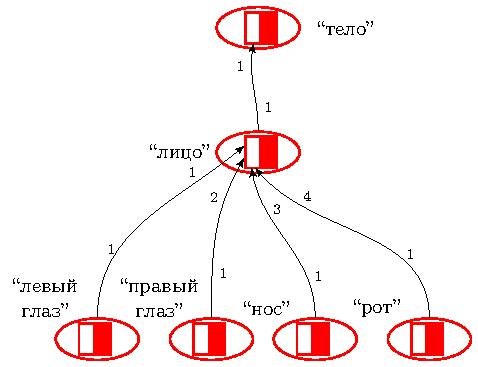
\includegraphics[width=0.5\textwidth,page=1]{examples/causnet/caus_net_colored}
		\caption{Пример каузальной сети на множестве образов знаков. Здесь каузальные матрицы изображены в виде квадратов, столбцы условий - левая белая часть квадрата, столбцы эффектов - черная правая часть квадратов. Метка $\epsilon_1$ отображается в начале каждой стрелки, метка $\epsilon_2$ определяется как номер квадрата, к которому идет стрелка, а метка $\epsilon_3$ отображается в конце каждой стрелки.}
		\label{fig:caus_net}		
	\end{figure}
		
	Аналогичным образом определяются каузальные сети для остальных компонент знака - для значения и личностного смысла. Для каждого знака $s$ задаются множества $S_m(s)$ и $S_a(s)$, т.е. определяются семейства вложенных отношений $\{\sqsubset_m,\sqsubset_m^1,\sqsubset_m^2,\dots\}$ - \textit{являться элементом значения}, и $\{\sqsubset_a,\sqsubset_a^1,\sqsubset_a^2,\dots\}$ - \textit{являться элементом смысла}. Множество $S_m(s)$ интерпретируется как ролевой состав знака $s$, например, элементы подкласса или роль действия, в соответствии с изложением семантического уровня модели. Множество $S_a(s)$ интерпретируется как мгновенный компонентный состав некоторой ситуации, наблюдаемой и переживаемой субъектом - носителем картины мира, или действия, совершаемого субъектом в настоящее время. Аналогично определяются множества $Z^m(s)$, $Z^a(s)$, процедуры $\Lambda_m$ и $\Lambda_a$.
	
	Три типа каузальных сетей отличаются друг от друга отношениями, которые генерируются на основе этих сетей для соответствующего множества компонент знаков, операциями, которые выполняются на этих сетях, и той ролью, которую они играют при реализации когнитивных функций, например, планирования поведения \cite{Osipov2015d,Panov2017a}. Теперь мы можем уточнить определение знака \cite{Osipov2015c} с использованием введенного формализма каузальных матриц и каузальных сетей.
	
	\begin{definition}
		Знаком будем называть четверку $s=\langle n, p, m, a \rangle$, где $n$ - имя знака, $p=Z^p$ - образ знака, т.е. кортеж каузальных матриц, которым соответствует некоторый узел каузальной сети на образах с учетом всех входящих и исходящих связей, $m=Z^m$ - значение знака, т.е. кортеж каузальных матриц, которым соответствует некоторый узел каузальной сети на значениях  с учетом всех входящих и исходящих связей, $a=Z^a$ - образ знака, т.е. кортеж каузальных матриц, которым соответствует некоторый узел каузальной сети на личностных смыслах  с учетом всех входящих и исходящих связей.
	\end{definition}
	
	Далее мы будем считать, что каждый знак обладает значением, т.е. $Z^m\not = \varnothing$. В том случае, когда у знака нет образа, т.е. $Z^p=\varnothing,S_p=\varnothing$, будем называть его \textit{знаком категории} (будем различать метапонятия и категории, как это указано в \cite{Osipov1997}). Наконец, в том случае, когда знаку не присвоен личностный смысл, т.е. $Z^a=\varnothing, S_a=\varnothing$, будем называть его \textit{безличным}.
	
	\section{Семиотическая сеть}\label{sec:semnetwork}
	
	Далее определим три семейства бинарных отношений на множестве знаков, которые  генерируются на основе структуры фрагментов трех типов каузальных сетей, к которым принадлежат соответствующие компоненты знаков. Эти отношения соответствуют отношениям, введенным на семантическом уровне.
		
	\subsection{Отношения на множестве образов}	
	
	Начнем с определения отношений на множестве знаков, генерируемых на основе каузальной сети на образах. Для этого потребуется определения равенства, сходства, включения и противопоставления двух каузальных матриц:
	
	\begin{definition}
		Две каузальных матрицы $z_1$ и $z_2$ равны ($z_1=z_2$) тогда и только тогда, когда размерности матриц равны, множества индексов столбцов эффектов и условий совпадают $\Lambda({z_1})=\Lambda({z_2})$ и каждый бинарный вектор $e_t^1$, столбец матрицы $z_1$, равен соответствующему по порядку бинарному вектору $e_t^2$, столбцу матрицы $z_2$.
	\end{definition}
	
	\begin{definition}
		Две каузальных матрицы $z_1$ и $z_2$ обладают сходством ($z_1\sim z_2$) тогда и только тогда, когда  существуют такие два бинарных вектора $e_i$ и $e_j$, столбца матриц $z_1$ и $z_2$, что их покомпонентное произведение (т.е. произведение тех компонент, которые соответствуют одному и тому же признаку, если соответствующего признака в векторе нет - считается, что на его месте стоит ноль) не равно нулевому вектору $e_i*e_j\not = 0$ и они одновременно являются либо столбцами условий $i\in I^c(z_1), j\in I^c(z_2)$, либо столбцами эффектов $i\in I^e(z_1), j\in I^e(z_2)$.
	\end{definition}
	
	\begin{definition}
		Каузальная матрица $z_1$ включена в каузальную матрицу $z_2$ ($z_1\subseteq z_2$) тогда и только тогда, когда  для любого бинарного вектора $e_i$, столбца матрицы $z_1$, существует бинарный вектор $e_j$, столбец матрицы $z_2$, такой, что $e_i | e_j=e_j$ ($|$ - операция побитового <<или>>) и они одновременно являются либо столбцами условий $i\in I^c(z_1), j\in I^c(z_2)$, либо столбцами эффектов $i\in I^e(z_1), j\in I^e(z_2)$.
	\end{definition}
	
	\begin{definition}
		Две каузальных матрицы $z_1$ и $z_2$ противопоставлены друг другу ($z_1\perp z_2$) тогда и только тогда, когда размерности матриц равны, множества индексов столбцов эффектов и условий совпадают $\Lambda({z_1})=\Lambda({z_2})$ и каждый бинарный вектор $e_t^1$, столбец матрицы $z_1$, не имеет пересечения с соответствующим ему по порядку бинарным вектором $e_t^2$, столбцом матрицы $z_2$, т.е. $e_t^1\& e_t^2=0$, где $\&$ - операция побитового <<и>>.
	\end{definition}
	
	Кроме уже введенного ранее семейства отношений <<являться элементом образа>> ${\sqsubset_p, \sqsubset_p^1, \dots}$, на основе определений отношений на множестве каузальных матриц, зададим четыре отношения на множестве знаков $S$.
	\begin{definition}
		Пара знаков  $s_1$ и $s_2$ принадлежит \textbf{отношению эквивалентности по образу} $R_{eq}^p$, $(s_1,s_2)\in R_{eq}^p$, если кортеж $Z^p(s_1)=\langle z_1^1,z_2^1,\dots\rangle$ поэлементно равен кортежу $Z^p(s_2)=\langle z_1^2,z_2^2,\dots\rangle$, т.е. их мощности равны и каждая каузальная матрица первого кортежа равна соответствующей матрице второго кортежа, т.е. $|Z^p(s_1)| = |Z^p(s_2)|, \forall z_t^1\in Z^p(s_1)\ \exists z_l^2\in Z^p(s_2): z_t^1=z_l^2, t=l$.
	\end{definition}
	
	\begin{definition}\label{def:sim}
		Пара знаков  $s_1$ и $s_2$ принадлежит \textbf{отношению сходства по образу} $R_{sim}^p$, $(s_1,s_2)\in R_{sim}^p$, если для каждой каузальной матрицы $z_i$ кортежа $Z^p(s_1)$ в кортеже $Z^p(s_2)$ найдется такая матрица $z_j$, что $z_i$ обладает сходством с $z_j$, т.е. $\forall z_i\in Z^p(s_1)\ \exists z_j\in Z^p(s_2): z_i\sim z_2$.
	\end{definition}
	
	\begin{definition}
		Пара знаков  $s_1$ и $s_2$ принадлежит \textbf{отношению включения по образу} $R_{in}^p$, $(s_1,s_2)\in R_{in}^p$, если для каждой каузальной матрицы $z_i$ кортежа $Z^p(s_1)$ в кортеже $Z^p(s_2)$ найдется такая матрица $z_j$, что $z_i$ будет включена в $z_j$, т.е. $\forall z_i\in Z^p(s_1)\ \exists z_j\in Z^p(s_2): z_i\subseteq z_2$.
	\end{definition}

	\begin{definition}
		Пара знаков  $s_1$ и $s_2$ принадлежит \textbf{отношению противопоставления по образу} $R_{con}^p$, $(s_1,s_2)\in R_{con}^p$, если мощность кортежа $Z^p(s_1)=\langle z_1^1,z_2^1,\dots\rangle$ равна мощности кортежа $Z^p(s_2)=\langle z_1^2,z_2^2,\dots\rangle$ и каждая каузальная матрица первого кортежа противопоставлена соответствующей матрице второго кортежа, т.е. $|Z^p(s_1)| = |Z^p(s_2)|, \forall z_t^1\in Z^p(s_1)\ \exists z_t^2\in Z^p(s_2): z_t^1\perp z_t^2$.
	\end{definition}
	
	Семейство отношений $R^p$ на множестве образов в виду введенных определений формируется отношениями <<являться элементом образа>>, эквивалентности, сходства, включения и противопоставления по образу.
		
	\subsection{Отношения на множестве значений}	
	
	К семейству отношений $R^m$ на множестве значений отнесем отношения <<являться элементом значения>> ${\sqsubset_m,\sqsubset_m^1,\dots}$ и аналогичные случаю с образами - отношения эквивалентности $R_{eq}^m$, сходства $R_{sim}^m$, включения $R_{in}^m$ и противопоставления $R_{con}^m$ по значению.
	
	Кроме того, важную роль на сети значений при моделировании когнитивных функций играют следующие два отношения: отношение классификации $R_{cl}^m$, причинно-следственное отношение $R_{cas}^m$ и сценарное отношение $R_{sc}^m$.

	
	\begin{definition}
		Пара знаков $s_1$ и $s_2$ принадлежит \textbf{отношению классификации} $R_{sc}^m$, $(s_1,s_2)\in R_{sc}^m$, если $s_1$ - объектный знак категории и существует только одна каузальная матрица значения знака $s_1$ с единственным столбцом, в котором только одна единица соответствует знаку $s_2$, т.е. $Z^p(s_1)=\varnothing, I^e(s_1)=\varnothing, \exists z\in Z^m(s_1): h(z)=1, |e_1(z)|=1, s_2\sqsubset_m^1 s_1$.
	\end{definition}
	
	\begin{definition}
		Пара знаков $s_1$ и $s_2$ принадлежит \textbf{сценарному отношению} $R_{cas}^m$, $(s_1,s_2)\in R_{}^m$, если $s_1$ - процедурный знак, $s_2$ - объектный знак, возможно, знак категории, и знак $s_2$ является элементом значения знака $s_1$, т.е. $I^e(s_1)\not = \varnothing, I^e(s_2) = \varnothing, s_2\sqsubset_m s_1$.
	\end{definition}
	
	Примеры элементов отношений $R_{cl}^m$ и $R_{sc}^m$ приведены на рис.\ref{fig:signif_relat}.


	\begin{figure}
		\centering
		\includegraphics[width=0.6\textwidth,page=2]{examples/causnet/caus_net_colored}
		\caption{Пример элементов отношений на каузальной сети значений. Здесь множество $\{(s_2,s_3),(s_2,s_4),(s_2,s_5),(s_2,s_6),(s_1,s_2)\}\subset R_{cl}^m$ интерпретируется как <<квадрат, треугольник, трапеция и круг являются геометрическими фигурами, которые выступают объектами действия рисовать>>. Множество $\{(s_7,s_1),(s_7,s_8),(s_7,s_9)\}\subset R_{sc}^m$ интерпретируется как <<действие рисовать задается ролями субъект (тот, кто рисует), инструмент (чем рисуют) и объект (что рисуют)>>. Условные обозначения те же, что и на рис.\ref{fig:caus_net}.}
		\label{fig:signif_relat}		
	\end{figure}
	
	\subsection{Отношения на множестве личностных смыслов}	
	К семейству отношений $R^a$ на множестве личностных смыслов отнесем отношения <<являться элементом смысла>> ${\sqsubset_a,\sqsubset_a^1,\dots}$ и аналогичные случаю с образами - отношения эквивалентности $R_{eq}^a$, сходства $R_{sim}^a$, включения $R_{in}^a$ и противопоставления $R_{con}^a$ по смыслу.
	
	Также на множестве личностных смыслов введем ситуационное отношение $R_{sit}^a$.

	\begin{definition}
		Пара знаков $s_1$ и $s_2$ принадлежит \textbf{ситуационному отношению} $R_{sit}^a$, $(s_1,s_2)\in R_{sit}^a$, если $s_1$ - процедурный знак, $s_2$ - объектный знак, не являющийся знаком категории, и знак $s_2$ является элементом смысла знака $s_1$, т.е. $I^e(s_1)\not = \varnothing, I^e(s_2) = \varnothing, S_p(s_2)=\varnothing, s_2\sqsubset_a s_1$.
	\end{definition}
	
	На основе определения ситуационного отношения оказывается возможным ввести понятия ситуации, определяемое на основе некоторого процедурного знака со всеми объектными знаками, не являющимися знаками категорий, в паре с которыми он принадлежит ситуационному отношению.
	
	\begin{definition}
		Множество знаков $Sit=\{s_1,s_2,\dots,s_n\}$ будем называть \textit{ситуацией}, если $s_1$ - единственный процедурный знак в множестве $Sit$ и для всех $1<i\leq n\ s_i\in Sit, (s_1,s_i)\in R_{sit}^a$.
	\end{definition}
	
	Пример элементов отношения $R_{sit}^a$ и ситуации приведен на рис.\ref{fig:mean_relat}

	\begin{figure}
		\centering
		\includegraphics[width=0.5\textwidth,page=3]{examples/causnet/caus_net_colored}
		\caption{Пример элементов отношения $R_{sit}^a$ на каузальной сети смыслов. Здесь множество $\{(s_5,s_1),(s_5,s_2),(s_5,s_3),(s_5,s_4)\}\subset R_{sit}^a$ эквивалентно ситуации <<Иван рисует трапецию карандашом>>. Условные обозначения те же, что и на рис.\ref{fig:caus_net}.}
		\label{fig:mean_relat}		
	\end{figure}
			
	\subsection{Семиотическая сеть}
	Будем называть \textit{семиотической сетью} пятерку $\Omega=\langle W_p, W_m, W_a, R, \Theta \rangle$, где
	\begin{itemize}
		\item $W_p, W_m, W_a$ - каузальные сети на множестве образов, значений и личностных смыслов, соответственно,
		\item $R$ - семейство отношений на множестве знаков, образованных на основе трех каузальных сетей, т.е. $R=\{R^p, R^m, R^a\}$,
		\item $\Theta$ - семейство операций на множестве знаков (которые будут определены ниже).
	\end{itemize} 
	

	\section{Структура операций в семиотической сети}\label{sec:operations}
	На структурном уровне модели картины мира уточним определения операций, которые функционируют в картине мира и генерируют новый знак либо сценарий на основе компонент двух входных знаков. Другими словами, генерация, например, нового образа на основе двух образов других знаков, влечет за собой формирование остальных компонент нового знака по  правилам данной операции. В настоящей работе для каждой каузальной сети в качестве примера будут даны определения тех из них, примеры которых на семантическом уровне были приведены в разд. \ref{sec:semantic}. Для простоты изложения будем далее считать, что каждая компонента знака характеризуется одной каузальной матрицей (одной действие, одно правило). Далее будет использована процедура образования нового знака, описанная в \cite{Osipov2014c}, которую здесь будем обозначать через $\Psi$.
	
	\subsection{Операция обобщения}
	
	Обобщение является одним из ключевых когнитивных процессов, которые позволяют организовывать знания в иерархической форме, формировать компактные представления объектов и процессов действительности. В психологии выделяют три вида обобщения: синкрет, комплекс и понятие \cite{Vygotsky1999}. При синкретическом обобщении ведущую роль играет личностный смысл знаков, т.е. субъективное отношение носителя картины мира к представляемым объектам. При формировании обобщения-комплекса используются образы знаков, объективно существующие признаки. Обобщение-понятие, основываясь на значении знаков, формируется уже в процессе рассмотрения родо-видовых отношений, знания о которых согласованы с другими участниками совместной деятельности.
	
	Определим операцию \textit{обобщения по образу} (образования обобщения-комплекса) $\Theta^p: S\times S\rightarrow S$. Пусть $s_1=\langle n_1, \{z_1^p\}, \{z_1^m\}, \{z_1^a\} \rangle$, $s_2=\langle n_2, \{z_2^p\}, \{z_2^m\}, \{z_2^a\} \rangle$ - знаки такие, что $(s_1,s_2)\in R_{eq}^p$, т.е. принадлежат отношению сходства. Новый образуемый знак обозначим через $s_3$. 
	
	По определению $\autoref{def:sim}$ это означает, что $z_1^p\sim z_2^p$, т.е. каузальные матрицы обладают сходством. Определим новую каузальную матрицу $z_3^p$ следующим образом: $z_3^p=(e_1^3,e_2^3,\dots,e_h^3)$, где для каждого столбца $e_i^3$ найдется пара столбцов $e_j^1, e_k^2$ матриц $z_1^p$ и $z_2^p$ соответственно, таких, что $e_i^3=e_j^1*e_k^2\not=\varnothing$ и $i\in I^c(z_3^p), j\in I^c(z_1^p), k\in I^c(z_2^p)$. Иными словами матрица $z_3^p$ является обобщением матриц $z_1^p$ и $z_2^p$ и содержит только те события, которые являются обобщением событий для обоих матриц.
	
	Пусть $Z'_1$ и $Z'_2$ - множества процедурных каузальных матриц, для которых знаки $s_1$ и $s_2$ соответственно являются признаками. Найдем среди этих двух множеств пару каузальных матриц, обладающих сходством: $(z_1^m,z_2^m)$. Далее определим процедурную каузальную матрицу $z_4^m$ - новую матрицу в каузальной сети значений, которая будет являться обобщением матриц $z_1^m$ и $z_2^m$: $z_4^m=(e_1^4,e_2^4,\dots)$, где для каждого столбца $e_i^4$ найдется пара столбцов $e_j^1, e_k^2$ матриц $z_1^m$ и $z_2^m$ соответственно, таких, что
	\begin{itemize}
		\item в каждом из них ссылка на соответствующие значения знаков $s_1$ и $s_2$ заменена на ссылку на значение c единственной пустой матрице $z_3^m$ вновь образуемого знака $s_3$,
		\item $e_i^4=e_j^1*e_k^2\not=\varnothing$ и 
		\item либо одновременно $i\in I^c(z_4^m), j\in I^c(z_1^m), k\in I^c(z_2^m)$, 
		\item либо одновременно $i\in I^e(z_4^m), j\in I^e(z_1^m), k\in I^c(z_2^m)$.
	\end{itemize}
	
	По сгенерированной паре матриц $z_3^p$ и $z_3^m$ с помощью процедуры образования нового знака $\Psi$ в результате операции $\Theta^p$ получаем новый знак $s_3$, образ которого является обобщением образов знаков $s_1$ и $s_2$, а значением является некоторая роль в обобщенном действии, выполняемом как со знаком $s_1$, так и со знаком $s_2$. Вновь образованная процедурная матрица $z_4^m$ может быть включена в один из существующих узлов на сети значений, либо послужить отдельным узлом нового знака, представляющего новое обобщенное действие.
	
	Приведем пример работы операции обобщения по образу. Пусть есть два знака $s_1$ и $s_2$ с именами \textit{<<яблоко>>} и \textit{<<апельсин>>} соответственно. Каузальные матрицы для образных компонент знаков $s_1$ и $s_2$ выглядят следующим образом (вместо единиц в матрице указаны имена признаков):
	\[
	z_1^p = \begin{bmatrix}
	0&0& \text{<<зеленый>>} \\
	0& \text{<<круглый>>} &0 \\
	\text{<<кожура>>} &0 &0  \\
	\text{<<тонкий>>} &0 &0
	\end{bmatrix}
	z_2^p = \begin{bmatrix}
	0&0& \text{<<оранжевый>>} \\
	0& \text{<<круглый>>} &0 \\
	\text{<<кожура>>} &0 &0  \\
	\text{<<толстый>>} &0 &0
	\end{bmatrix}
	\]
	Компоненты значений знаков $s_1$ и $s_2$ связаны по каузальной сети с процедурными знаками $s_3$ <<чистить яблоко>> и $s_4$ <<чистить апельсин>> (здесь вертикальной чертой отделены столбцы условий и эффектов):
	\[
	z_3^m= \left[\begin{array}{ccc|cccc}
	0&0&0&0&\text{<<стол>>}&0\\
	0&\text{<<яблоко>>}&0& 0&0&\text{<<яблоко>>}\\
	0&0& \text{<<нож>>} &0 &0\\
	0& 0& 0 &\text{<<на>>} &0&0\\
	\text{<<вплотную>>}& 0& 0 &0 &0&0\\
	\text{<<кожура>>} &0 &0 &\text{<<кожура>>}  &0&0\\
	\text{<<тонкий>>} &0 &0 & \text{<<тонкий>>} &0&0
	\end{array}
	\right]
	\]
	\[
	z_4^m= \left[\begin{array}{ccc|cccc}
	0&0&0&0&\text{<<стол>>}&0\\
	0&\text{<<апельсин>>}&0& 0&0&\text{<<апельсин>>}\\
	0&0& \text{<<пальцы>>} &0 &0&0\\
	0& 0& 0 &\text{<<на>>} &0&0\\
	\text{<<вплотную>>}& 0& 0 &0 &0&0\\
	\text{<<кожура>>} &0 &0 &\text{<<кожура>>}  &0&0\\
	\text{<<толстый>>} &0 &0 & \text{<<толстый>>} &0&0
	\end{array}
	\right]
	\] 
	В результате выполнения операции обобщения по образу $\Theta^p$ формируются два знака: обобщенный по признакам образа знак $s_5$ с именем <<фрукт>> и обобщенный по признакам значения знак $s_6$ чистить, представляющий собой обобщенное действие, которое можно выполнить с фруктом:
	
	\[
	z_5^p = \begin{bmatrix}
	0& \text{<<круглый>>} \\
	\text{<<кожура>>} &0
	\end{bmatrix}
	\]
	\[
	z_6^m= \left[\begin{array}{ccc|cccc}
	0&0&0&0&\text{<<стол>>}&0\\
	0&\text{<<фрукт>>}&0& 0&0&\text{<<фрукт>>}\\
	0& 0& 0 &\text{<<на>>} &0&0\\
	\text{<<вплотную>>}& 0& 0 &0 &0&0\\
	\text{<<кожура>>} &0 &0 &\text{<<кожура>>}  &0&0\\
	\end{array}
	\right]
	\] 
	
	\subsection{Операция замыкания по значению}
	Другой важной когнитивной функцией является способность формировать возможные сценарии на основе значений знаков. Особую роль этот процесс играет в житейской картине мира, где большинство когнитивных процессов, формирующих поведение человека, таких как планирование, коммуникация, основываются на нахождении, применении и образовании новых сценариев \cite{Chudova2012b,Osipov2015d}. Под сценарием в простейшем случае подразумевается некоторое действие, в котором зафиксированы исполнители той или иной роли, т.е. сценарий является специфицированным действием. Формально сценарием будем называть множество знаков $Scen=\{s_1,s_2,\dots, s_n\}$, в котором единственным процедурным знаком является $s_1$, а все остальные знаки образуют две подгруппы $S_r$ - множество знаков-ролей и $S_o$ - множество знаков-участников сценария. Знаки-роли из множества $S_r$ - это знаки категорий, которые связаны с $s_1$ сценарным отношением $R_{sc}^m$. Знаки-участники из множества $S_o$ - это либо не знаки, не являющиеся знаками категорий, связанные с $s_1$ сценарным отношением $R_{sc}^m$, либо знаки, которые в паре с другим знаком из множества $S_r$ принадлежат отношению классификации $R_{cl}^m$.
	
	Определим операцию \textit{замыкания по значению} $\Theta^m$, которая по некоторому процедурному знаку $s$ формирует сценарий $Scen$: $\Theta^m(s)=Scen$. По сути формирование сценария заключается в итерационном включении знаков в множество $Scen$ при рассмотрении элементов отношений $R_{cl}^m$ и $R_{sc}^m$:
	
	\begin{itemize}
		\item[Шаг 1.] Включить в сценарий $Scen$ процедурный знак $s$: $Scen=\{s\}$.
		\item[Шаг 2.] Пополнить сценарий знаками, которые связаны с $s_1$ сценарным отношением: $Scen=Scen\cup\{s_i|(s_1,s_i)\in R_{sc}^m, I^e(s_i)=\varnothing\}$.
		\item[Шаг 3.] Пополнить сценарий знаками, не являющимися знаками категорий, который связаны с объектными знаками сценария отношением классификации: $Scen=Scen\cup\{s_j|(s_i,s_j)\in R_{cl}^m, s_i\in Scen, I^e(s_i)=\varnothing, S_p(s_i)=\varnothing, S_p(s_j)\not=\varnothing\}$.
		\item[Шаг 4.] Повторять шаг 3 до тех пор, пока сценарий не перестанет пополняться новыми знаками либо не будут перебраны все знаки из некоторого множества, определяемого решаемой задачей. Например, при решении задачи целеполагания, используется только некоторое подмножество знаков, кандидатов в образуемый сценарий \cite{Osipov2014c}.
	\end{itemize}
	
	Пример сформированного сценария представлен рис.\ref{fig:scenarion}.
	
	\begin{figure}
		\centering
		\includegraphics[width=0.8\textwidth,page=4]{examples/causnet/caus_net_colored}
		\caption{Пример сценария. Центральный процедурный знак - $s_5$. Знаки-роли $S_r=\{s_1,s_2,s_3,s_4\}$, знаки-участники $S_o=\{s_7,s_8,s_9,s_{10},s_{11}\}$. Элементы сценарного отношения обозначены сплошными стрелками, отношения классификации - прерывистыми. Остальные условные обозначения те же, что и на рис.\ref{fig:caus_net}.}
		\label{fig:scenarion}		
	\end{figure}

		
	\subsection{Операция агглютинации смыслов}
	
	В заключение приведем характерный пример операции на сети личностных смыслов - операции агглютинации. Агглютинация, или слияние, смыслов двух знаков позволяет сформировать новый смысл у третьего знака, обычно, уже существующего в картине мира. В психологии новый смысл представляет собой комбинацию, сочетание данных в опыте элементов, что представляет собой один из основных механизмов воображения и творческой деятельности \cite{Asmolov1990,Rubinshtain2000}. Примером слияния смыслов в искусстве могут служить аллегорические фигуры Леонардо да Винчи, а в лингвистике - такие слова как <<Мойдодыр>> или <<Айболит>>.
	
	Используя введенный формализм, определим операцию агглютинации $\Theta^a$: $S\times S\rightarrow S$. Пусть $s_1=\langle n_1, \{z_1^p\}, \{z_1^m\}, \{z_1^a\} \rangle$, $s_2=\langle n_2, \{z_2^p\}, \{z_2^m\}, \{z_2^a\} \rangle$. Образуемый или уже существующий в картине мира знак обозначим через $s_3$. В результате выполнения операции $\Theta^a$ у знака $s_3$ образуется новый смысл, представляемый каузальной матрицей $z_3^a$, которая строится следующим образом. Пусть $z_1^a=(e_1^1, e_2^1,\dots,e_h^1)$ и $z_2^a=(e_1^2, e_2^2,\dots,e_l^2)$, тогда каузальная матрица $z_3^a=(e_1^3, e_2^3,\dots,e_q^3)$, где $q=h+l$, $I^c(z_3^a)=I^c(z_1^a)\cup \{i+|I^c(z_1^a)||i\in I^c(z_2^a)\}$, $I^e(z_3^a)=I^e(z_1^a)\cup \{i+|I^e(z_1^a)||i\in I^e(z_2^a)\}$, а 
	\[
		e_t^3=\begin{cases}
		e_t^1, &\text{если}\ t<|I^c(z_1^a)|,\\
		e_{t-|I^c(z_1^a)|}^2, &\text{если}\ |I^c(z_1^a)|<t<|I^c(z_1^a)|+|I^c(z_2^a)|,\\
		e_{t-|I^c(z_2^a)|}^1, &\text{если}\ |I^c(z_1^a)|+|I^c(z_2^a)|<t<|I^c(z_1^a)|+|I^c(z_2^a)|+|I^e(z_1^a)|,\\
		e_{t-|I^c(z_1^a)|-|I^e(z_1^a)|}^2, &\text{если}\ t>|I^c(z_1^a)|+|I^c(z_2^a)|+|I^e(z_1^a)|.
		\end{cases}
	\]
	Переходя к нотации правил, мы можем сказать, что новый смысл, представляемый правилом $z_3^a$, является объединением условий и эффектов правил $z_1^a$ и $z_2^a$: $F_C(z_3^a)=F_C(z_1^a)\cup F_C(z_2^a)$ и либо $F_A(z_3^a)=F_A(z_1^a)\cup F_A(z_2^a)$, либо $F_D(z_3^a)=F_D(z_1^a)\cup F_D(z_2^a)$ \cite{Osipov2016a}.
	
	В качестве примера приведем образование нового личностного смысла у знака <<Санкт-Петербург>> в результате операции агглютинации смыслов знаков <<газета>> и <<кофе>>, представимых в виде следующих матриц (действия <<читать газету>> <<пить кофе>>):
	\[
	z_1^a= \left[\begin{array}{ccc|cccc}
	0&0&0&0&0&0&\text{<<новости>>}\\
	0&\text{<<кафе>>}&0&0&\text{<<кафе>>}&0&0\\
	0&\text{<<на>>}&0&0 &\text{<<на>>}&0&0\\
	0& 0& \text{<<Невский>>}&0 &0&\text{<<Невский>>}&0\\
	\text{<<газета>>}&0&0&\text{<<газета>>}&0&0&0\\
	\text{<<в>>} &0 &0 &\text{<<в>>}&0&0&0\\
	0&0 &0 & 0 &0&0&0
	\end{array}
	\right]
	\]
	\[
	z_2^a= \left[\begin{array}{ccc|cccc}
	0&0&0&0&0&0&\text{<<кофе>>}\\
	0&\text{<<кафе>>}&0&0&\text{<<кафе>>}&0&0\\
	0&\text{<<на>>}&0&0 &\text{<<на>>}&0&0\\
	0& 0& \text{<<Невский>>}&0 &0&\text{<<Невский>>}&0\\
	\text{<<чашка>>}&0&0&\text{<<газета>>}&0&0&0\\
	\text{<<в>>} &0 &0 &\text{<<в>>}&0&0&0\\
	0&0 &0 & 0 &0&0&0
	\end{array}
	\right]
	\] 
	Новая каузальная матрица $z_3^a$ будет выглядеть следующим образом. Столбцы условий являются последовательным объединением столбцов-условий матриц $z_1^a$ и $z_2^a$ (лишние строчки нулей опущены)
	\[
	\left[\begin{array}{cccccc}
	0&\text{<<кафе>>}&0&0&\text{<<кафе>>}&0\\
	0&\text{<<на>>}&0&0 &\text{<<на>>}&0\\
	0& 0& \text{<<Невский>>}&0 &0&\text{<<Невский>>}\\
	\text{<<газета>>}&0&0&0&0&0\\
	0&0&0&\text{<<чашка>>}&0&0\\
	\text{<<в>>} &0 &0 &\text{<<в>>}&0&0
	\end{array}
	\right]
	\]
	Столбцы эффектов являются последовательным объединением столбцов эффектов матриц $z_1^a$ и $z_2^a$ (лишние строчки нулей опущены)
	\[
	\left[\begin{array}{cccccccc}
	0&0 &0 &\text{<<новости>>}&0&0&0&0\\
	0&0 &0 &0&0&0&0&\text{<<кофе>>}\\	
	0&\text{<<кафе>>}&0&0&0&\text{<<кафе>>}&0&0\\
	0&\text{<<на>>}&0&0&0 &\text{<<на>>}&0&0\\
	0& 0& \text{<<Невский>>}&0&0 &0&\text{<<Невский>>}&0\\
	\text{<<газета>>}&0&0&0&0&0&0&0\\
	0&0&0&0&\text{<<чашка>>}&0&0&0\\
	\text{<<в>>} &0 &0&0&\text{<<в>>}&0&0&0
	\end{array}
	\right]
	\]
	
	В данном случае вопрос выбора знака $s_3$, у которого образуется новый смысл, мы не рассматриваем.
	
	\section*{Заключение}
	В работе представлен новый подход к интеграции знаний субъекта деятельности о внешней среде и своих характеристиках и к рассмотрению операций на основе этих знаний - знаковая картина мира. Дано описание модели картины мира на синтаксическом, семантическом и структурном уровнях. Использовано четырхекомпонентное понятие знака, введенное в предыдущих работах авторов на основе нейрофизиологических и психологических соображений. Введена специальная математическая структура - каузальная матрица, которая интегрирует в себе представление как статической информации в виде множества признаков, так и процедурной информации в виде правила с эффектами и условиями. Введено три типа семантических сетей на основе множества каузальных матриц - каузальные сети на образах, значениях и личностных смыслах. С использованием представленного формализма удается построить алгоритмы пополнения отношений на множестве знаков, моделирующих основные связи объектов и процессов внешнего мира. В работе описаны важные операции в картине мира, которые моделируют ключевые когнитивные функции - обобщение, формирование сценариев и агглютинацию смыслов.
	
	\printbibliography
\end{document}